
\chapter{Installation of model engines} \label{chap:install}
\renewcommand{\tabdir}{chapters/install/install/tab}
\renewcommand{\figdir}{chapters/install/install/fig}

\section{Introduction} \label{sec:install:intro}

This chapter deals with the installation of \software{echse}-based model engines from \emph{existing} source code. The chapter does not cover the topic of model development or modification. The information is addressed to users of both Linux and Windows.

In this context, the term \emph{model engine} is used to denote the binary file which is executed when performing a simulation. The term is introduced to allow for a clear distinction between the \emph{model engine} (plain binary file) and the \emph{model} (binary file + input data). 

%%%%%%%%%%%%%%%%%%%%%%%%%%%%%%%%%%%%%%%%%%%%%%%%%%%%%%%%%%%%%%%%%%%%%%%%%%%%%%
%%%%%%%%%%%%%%%%%%%%%%%%%%%%%%%%%%%%%%%%%%%%%%%%%%%%%%%%%%%%%%%%%%%%%%%%%%%%%%

\section{Software to install} \label{sec:install:software}

%%%%%%%%%%%%%%%%%%%%%%%%%%%%%%%%%%%%%%%%%%%%%%%%%%%%%%%%%%%%%%%%%%%%%%%%%%%%%%

\subsection{Programs}

You need to install the following programs in order to build an \software{echse}-based model engine:

\begin{itemize}
  \item The 'R' software for statistical computing.
  \item The GNU C++ compiler 'g++'.
  \item Windows users: The bash-shell interpreter and commands provided by 'MSYS'.
\end{itemize}

Linux users probably want to use the package manager to install the software. Windows users should try the installers which can be downloaded from the respective websites. Please follow the installation instructions given in \chapref{chap:extSoft} as closely as possible. In particular, on Windows systems, it is important to add the binary directories of all the software to the \verb!PATH! variable in order to make the programs accessible from any shell.

%%%%%%%%%%%%%%%%%%%%%%%%%%%%%%%%%%%%%%%%%%%%%%%%%%%%%%%%%%%%%%%%%%%%%%%%%%%%%%

\subsection{R-packages}

You need to install the R-package \software{codegen} in order to run the \software{echse}'s code generator. You should find the latest version of this package in the sub-folder \verb!R/packages! of the \software{echse}-tools main directory (see \secref{sec:install:folders}). The package is distributed as a tarball archive \verb!codegen_x.y.tar.gz! where \verb!x.y! is the current version number. See \secref{sec:extSoft:R:packages} for details on how to install R-packages.

%%%%%%%%%%%%%%%%%%%%%%%%%%%%%%%%%%%%%%%%%%%%%%%%%%%%%%%%%%%%%%%%%%%%%%%%%%%%%%
%%%%%%%%%%%%%%%%%%%%%%%%%%%%%%%%%%%%%%%%%%%%%%%%%%%%%%%%%%%%%%%%%%%%%%%%%%%%%%

\section{The \software{echse} standard folders} \label{sec:install:folders}

%%%%%%%%%%%%%%%%%%%%%%%%%%%%%%%%%%%%%%%%%%%%%%%%%%%%%%%%%%%%%%%%%%%%%%%%%%%%%%

\subsection{Overview} \label{sec:install:folders:overview}

At present, all \software{echse}-related files are split accross a small number of folders, also referred to as the \software{echse} \emph{standard folders}. These folders are briefly explained in \tabref{tab:install:folders}.

\begin{table}[h]
  \caption{The \software{echse} standard folders. \label{tab:install:folders}}  
  \begin{tabular}{p{0.2\textwidth}p{0.75\textwidth}} \hline\hline
     Folder & Contents \\ \hline
     \verb!echse_docs! & Documentations, mostly as \LaTeX{} projects. \\
     \verb!echse_generic! & Common C++ source code being used by all \software{echse}-based model engines. Also contains generic scripts for engine building. \\
     \verb!echse_engines! & C++ source code of the classes being used by one or more particular model engines. This includes both generated and manually written code. Also contains text files with class and model declarations. \\
     \verb!echse_tools! & \software{echse}-related tools for pre- and post-processing of data. \\
     \hline\hline
  \end{tabular}
\end{table}

It is assumed that you have obtained current versions of the \software{echse} standard folders listed in \tabref{tab:install:folders} either from repositories or by unpacking release archives. In order to install a model engine, you need at least the \verb!echse_generic! and \verb!echse_engines! folders whose contents is displayed in \figsref{fig:install:folders:generic} \& \ref{fig:install:folders:engines}, respectively. Note that only the most important branches are displayed in these figures.

\begin{figure}[h]
\begin{lstlisting}[style=text]
  echse_generic --+-- core
                  |
                  +-- cpplib
                  |
                  +-- scripts
\end{lstlisting}
  \caption{Main branches of the \software{echse} standard folder with generic files. \label{fig:install:folders:generic}}
\end{figure}

\begin{figure}[h]
\begin{lstlisting}[style=text]
  echse_engines --+-- bin
                  |
                  +-- classes
                  |
                  +-- def
                  |
                  +-- generated
                  |
                  +-- processes
\end{lstlisting}
\caption{Main branches of the \software{echse} standard folder with class files for particular model engines. \label{fig:install:folders:engines}}
\end{figure}

The functionality of many scripts and files contained in the folders \verb!echse_generic! and \verb!echse_engines! and its sub-folders depends on the integrity of the respective directory trees. Therefore, you should \emph{not} rename, move, or delete any of the sub-folders and files without considering the potential consequences. Note that all references to files and directories are \emph{relative}. Therefore, you can savely move each of the \software{echse} standard folders \emph{as a whole} as long as you keep your system informed on their locations (see \secref{sec:install:env:folders}).

%%%%%%%%%%%%%%%%%%%%%%%%%%%%%%%%%%%%%%%%%%%%%%%%%%%%%%%%%%%%%%%%%%%%%%%%%%%%%%

\subsection{Definition of model engines} \label{sec:install:folders:engines}

The following enumeration outlines the concept of model engines from a top-down point of view. It also gives a brief overview of the contents of the \software{echse} standard folder \verb!echse_engines!.

\begin{enumerate}
  \item Each model engine is composed of a particular set of classes. A rainfall-runoff model, for example, may comprise a sub-basin class, a reach class, and additional classes for special types of objects (reservoirs etc.). The set of classes being used in a particular model engines is listed in the text files in folder \verb!echse_engines/def!.
  \item Each of the classes is characterized by a particular set of data members (forcings, state variables, parameters, etc.). For each class, the declaration of data members can be found in the text files in folder \verb!echse_engines/classes/declaration!. See \citet{Echse-Main-Doc} for details.
  \item Class declaration and implementation are well separated. The declaration part of the classes' source code is created by the code generator (output in \verb!echse_engines/generated!). The implementation part consisting of manually written code to be found in \verb!echse_engines/classes/implementation! (C++ include files).
  \item The dynamics of state variables are due to the action of processes. In the \software{echse} concept, processes are represented by functions whose return value is typically a rate (mass or energy flux) or a derivative of a state variable with respect to time. Since a particular function may be used in multiple classes, the code is separated from the class implementation. It can be found in \verb!echse_engines/processes!
\end{enumerate}

%%%%%%%%%%%%%%%%%%%%%%%%%%%%%%%%%%%%%%%%%%%%%%%%%%%%%%%%%%%%%%%%%%%%%%%%%%%%%%
%%%%%%%%%%%%%%%%%%%%%%%%%%%%%%%%%%%%%%%%%%%%%%%%%%%%%%%%%%%%%%%%%%%%%%%%%%%%%%

\section{Environment variables to be set} \label{sec:install:env}

\subsection{Pointers to the \software{echse} standard folders} \label{sec:install:env:folders}
The \software{echse} is not a software in the classical sense and, therefore, it does not require the typical installation procedure. There is neither an installer nor is the \software{echse} distributed as an installable software package. In particular, on a Windows system, the \software{echse} does not integrate into the so-called 'registry'.

Any \software{echse}-related files are contained in the standard folders introduced in \secref{sec:install:folders}. All you need to do is to inform the system on the location of these folders. For that purpose, you must define the environment variables listed in \tabref{tab:install:env:folders}. Note that the variable names are UPPERCASE. See \appref{chap:appendix:envVars} and/or the help files of your operating system for detailed information on how to permanently set environment variables.

\begin{table}[h]
  \caption{Environment variables pointing to the \software{echse} standard folders. \label{tab:install:env:folders}}
  \begin{tabular}{p{0.2\textwidth}p{0.75\textwidth}} \hline\hline
    Variable name & Value \\ \hline
    \verb!ECHSE_GENERIC! & Full path of the \software{echse} standard folder \verb!echse_generic!. \\
    \verb!ECHSE_ENGINES! & Full path of the \software{echse} standard folder \verb!echse_engines!. \\
    \verb!ECHSE_TOOLS! & Full path of the \software{echse} standard folder \verb!echse_tools!. \\
    \hline\hline
  \end{tabular}
\end{table}

\begin{minipage}{0.15\textwidth}
  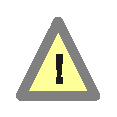
\includegraphics[width=0.6\textwidth]{../../_common/fig/symbols_warning.eps}   
\end{minipage}
\begin{minipage}{0.8\textwidth}
On Windows systems, you need to use the forward slash (\verb!/!) instead of the usual back-slash (\verb!\!) to separate directory names in the value of the environment variables listed in \tabref{tab:install:env:folders}. For example, if one of your \software{echse} standard folders is \verb!d:\modeling\echse_generic!, the proper value of \verb!ECHSE_GENERIC! would be \verb!d:/modeling/echse_generic!. Disregard of this will cause problems during the compilation of model engines.
\end{minipage} \\

\begin{minipage}{0.15\textwidth}
  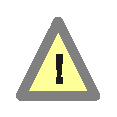
\includegraphics[width=0.6\textwidth]{../../_common/fig/symbols_warning.eps}   
\end{minipage}
\begin{minipage}{0.8\textwidth}
There must be no white space characters in the names of the \software{echse} standard folders. The existence of such characters (at any position) would break the functionality of some scripts. If you care for readability, use the \verb!_! character instead of white space, \ie{} use \verb!d:/my_files/echse_generic! instead of \verb!d:/my files/echse_generic!, for example. Disregard of this will cause problems during the compilation of model engines.
\end{minipage} \\

If you ever move one (or all) of the \software{echse} standard folder(s), the variables listed in \tabref{tab:install:env:folders} need to be updated to reflect the new location(s). If you follow the recommendations in \secref{sec:install:env:path}, no additional work is necessary.

\subsection{Adjusting the PATH variable} \label{sec:install:env:path}

Some sub-directories of the \software{echse} standard folders contain executable files (binaries and shell scripts). This is true in particular for the two folders \verb!echse_engines/bin! (\figref{fig:install:folders:engines}) and \verb!echse_generic/scripts! (\figref{fig:install:folders:generic}). It is recommended to add these two folders to the \verb!PATH! environment variable. Only then you will be able to run \software{echse}-based model engines as well as code generation and build scripts from any terminal without typing full path names.

It is strongly recommended that you make use of the already-defined environment variables \verb!ECHSE_ENGINES! and \verb!ECHSE_GENERIC! when adding these folders to \verb!PATH!. Then you can move the \software{echse} standard folders without updating \verb!PATH! again. For example, Linux users should could add the following line to their shell initialization file (see also \appref{chap:appendix:envVars}):

\begin{lstlisting}[style=shell]
  export PATH=$PATH:$ECHSE_ENGINES/bin:$ECHSE_GENERIC/scripts
\end{lstlisting}

Windows users need to adjust the settings in an equivalent way using the control panel. For example, the variable \verb!PATH! could have a contents similar to this one:
\begin{lstlisting}[style=shell]
  c:\mingw\bin;
  c:\mingw\msys\1.0\bin;
  c:\program files\R\R-2.15.2\bin;
  %ECHSE_GENERIC%\scripts;
  %ECHSE_ENGINES%\bin
\end{lstlisting}

Note that, to make this work, the \verb!PATH! variable being set must be of the same category as the referenced variables \verb!ECHSE_GENERIC! and \verb!ECHSE_ENGINES!. This is due to the fact that a \emph{user}-variable cannot be referenced in the definition of a \emph{system}-variable and vice versa. Therefore, users without administrator privileges usually need to define a user-variable \verb!PATH! in addition to the existing system-variable with that name.

%%%%%%%%%%%%%%%%%%%%%%%%%%%%%%%%%%%%%%%%%%%%%%%%%%%%%%%%%%%%%%%%%%%%%%%%%%%%%%
%%%%%%%%%%%%%%%%%%%%%%%%%%%%%%%%%%%%%%%%%%%%%%%%%%%%%%%%%%%%%%%%%%%%%%%%%%%%%%

\section{Building a model engine} \label{sec:install:build}

\subsection{Pre-requisites}

To be successsful, you should have read the sections \secsref{sec:install:folders}, \ref{sec:install:env}, and \ref{sec:install:software}. It is recommended that you perform some basic checks at a terminal prompt to make sure that the environment variable(s) are defined as intended and that the required software works properly.

\subsection{Run the code generator}
The code generator must be run from a shell prompt. On a Linux system, type the command \verb!echse_generate! followed by a space and the name of the model engine for which code is to be generated.

\medskip
\begin{minipage}{0.3\textwidth}
  Example:
\end{minipage}
\begin{minipage}{0.6\textwidth}
\begin{lstlisting}[style=shell]
  david@falkenstein:~$ echse_generate myEngine
\end{lstlisting}
\end{minipage}

On a Windows system, use the command  \verb!echse_generate_win.bat! instead of \verb!echse_generate!.

\medskip
\begin{minipage}{0.3\textwidth}
  Example:
\end{minipage}
\begin{minipage}{0.6\textwidth}
\begin{lstlisting}[style=shell]
  d:\> echse_generate_win.bat myEngine
\end{lstlisting}
\end{minipage}

\medskip
To make the commands work at any prompt, the folder \verb!echse_generic/scripts! (\figref{fig:install:folders:generic}) must be part of the \verb!PATH! variable (see \secref{sec:install:env:path}).

The scripts provide some basic error checking. In most cases, you should be able to fix the problem yourself. Note that you can only generate code for model engines that have already been designed (by declaring the classes).

\subsection{Run the build script}
The build script must be run from a shell prompt. On a Linux system, type the command \verb!echse_build! followed by a space and the name of the model engine. If want to skip the re-build of the static C++ library in order to speed up the compilation, you can set the second argument to 'n' (see example below). Use this option only if the library was just updated and note the warnings below.

\medskip
\begin{minipage}{0.3\textwidth}
  Examples:
\end{minipage}
\begin{minipage}{0.6\textwidth}
\begin{lstlisting}[style=shell]
  david@falkenstein:~$ echse_build myEngine
  david@falkenstein:~$ echse_build myEngine n
\end{lstlisting}
\end{minipage}

On a Windows system, use the command  \verb!echse_build_win.bat! instead of \verb!echse_build!.

\medskip
\begin{minipage}{0.3\textwidth}
  Examples:
\end{minipage}
\begin{minipage}{0.6\textwidth}
\begin{lstlisting}[style=shell]
  d:\> echse_build_win.bat myEngine
  d:\> echse_build_win.bat myEngine n
\end{lstlisting}
\end{minipage}

\medskip
To make the commands work at any prompt, the folder \verb!echse_generic/scripts! (\figref{fig:install:folders:generic}) must be part of the \verb!PATH! variable (see \secref{sec:install:env:path}).

\medskip
\begin{minipage}{0.15\textwidth}
  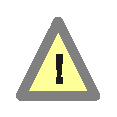
\includegraphics[width=0.6\textwidth]{../../_common/fig/symbols_warning.eps}   
\end{minipage}
\begin{minipage}{0.8\textwidth}
The C++ library \verb!libcpplib.a! is platform-specific, \ie{} you cannot re-use the file when switching between operating systems and/or compiler versions. Disregard of this may yield an executable with subtile bugs which are very hard to trace. Thus, the library must always be re-build after a new installation of the \software{echse} software and each time the C++ compiler is upgraded. The re-build should only be skipped if you run a sequence of attempts to build a model engine and compile time really matters.
\end{minipage} \\

The build scripts provide some basic error checking. If yout get rather lengthy error messages, possible several pages, this indicates a compiler problem. Please make sure that (1) you have the complete source code for the model engine you try to build, (2) the code generator ran without reporting errors, (3) the C++ library was re-build, and (4) the C++ compiler is properly installed.

